\appendix
\addappheadtotoc
\chapter{Code}
\label{apdx:code}
The following sections include the code used.  It was written for Matlab R2011b and requires SPM8 to run.  Additionally, it is recommended that you have at least 4 GB of RAM in order to work with the large datasets that are produced.  For information about how to visualize the data produced, see~\cref{apdx:visualize}.  All of the code is available through the temptools github page (\url{https://github.com/greggroth/temptools}).  Additionally, many of the tasks can be completed using the temptools gui (\cref{fig:ttmain,fig:ttcalcequil,fig:tttempcalc,fig:ttvisualize}) which can be invoked by running
\begin{lstlisting}[style=snippet]
  temptools
\end{lstlisting}
at the Matlab command prompt (make sure the temptools directory and subdirectories have been added to the Matlab path).  The procedure used is explained in~\cref{sec:approach} and a graphical representation is available in~\cref{fig:procedureflowchart}.
\begin{figure}[hbt]
  \centering
    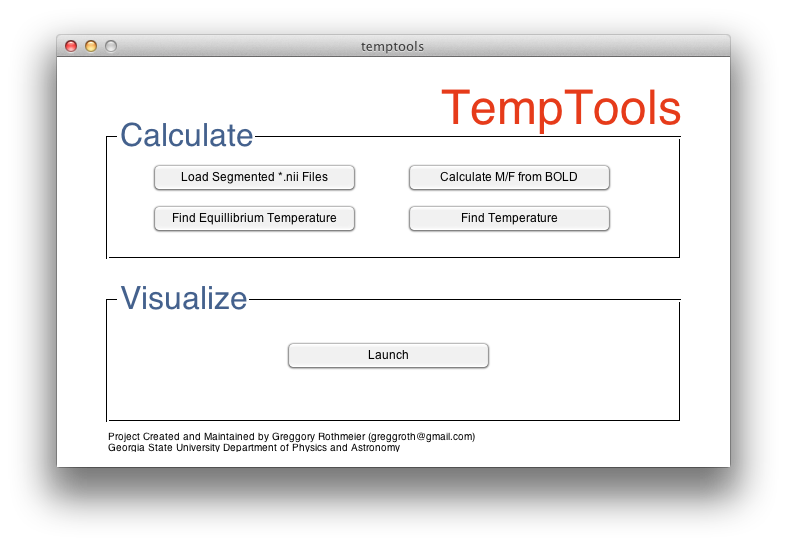
\includegraphics[keepaspectratio=true, width=17cm]{temptools/main.png}
    \caption[temptools: main window]{\label{fig:ttmain} The main window of temptools.  From here, you can go through the calculation steps and launch the visualization tool.}
  \centering
\end{figure}
\begin{figure}[hbt]
  \centering
    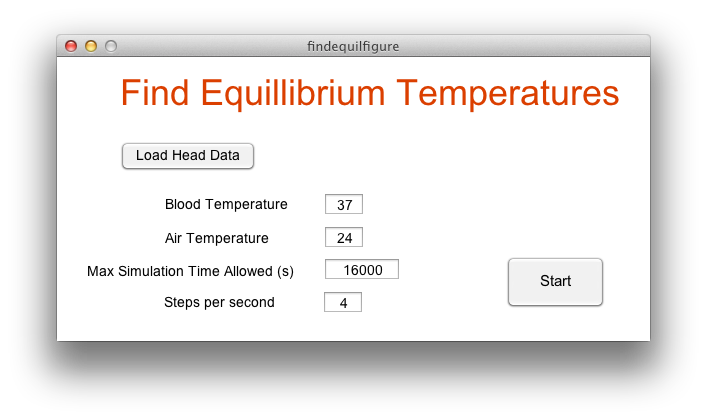
\includegraphics[keepaspectratio=true, width=17cm]{temptools/calcequil}
    \caption[temptools: calculate the equilibrium temperature window]{\label{fig:ttcalcequil} This is the interface for calculating the equilibrium temperature (method explained in~\cref{apdx:findequil}) under certain conditions.}
  \centering
\end{figure}
\begin{figure}[hbt]
  \centering
    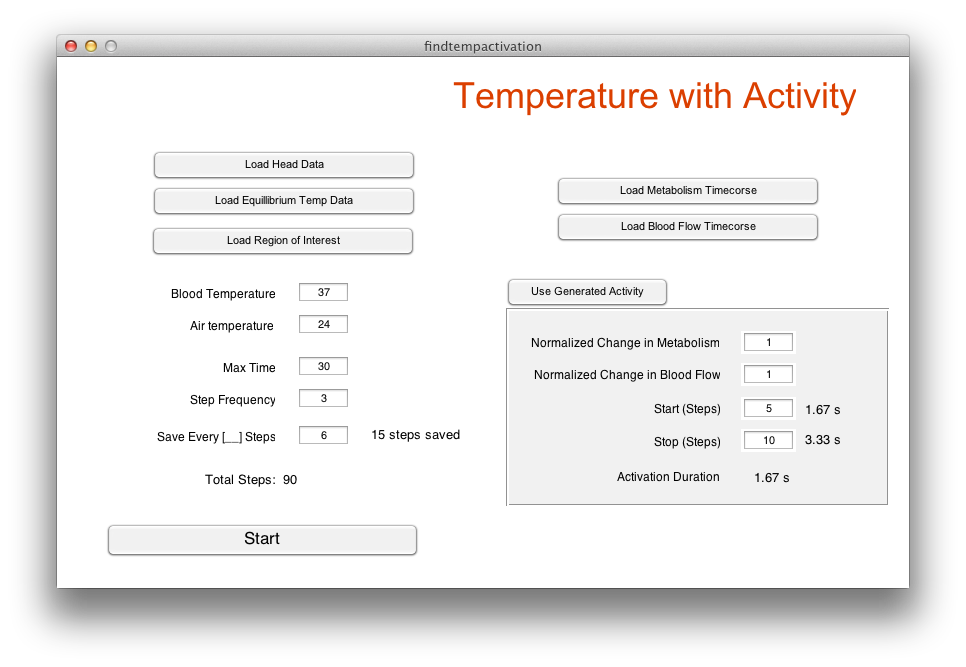
\includegraphics[keepaspectratio=true, width=17cm]{temptools/tempcalc}
    \caption[temptools: calculate temperature during activity]{\label{fig:tttempcalc} The interface for calculating temperature changes when blood flow and metabolism are time dependent.  This can be achieved by either loading metabolism and blood flow datasets or by using generated activity.}
  \centering
\end{figure}
\begin{figure}[hbt]
  \centering
    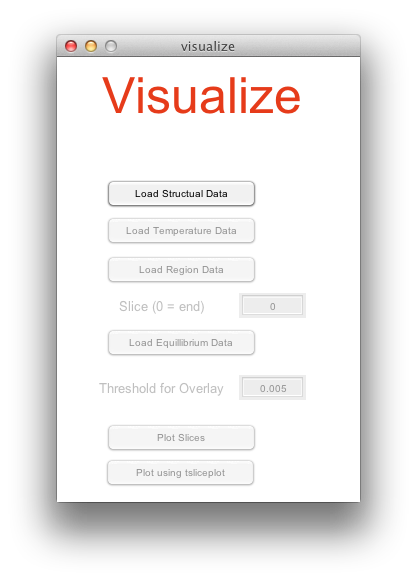
\includegraphics[keepaspectratio=true, width=10cm]{temptools/visualize}
    \caption[temptools: visualize the data]{\label{fig:ttvisualize} Visualize your data using the temptools visualization window.  This loads all of the required data and launches a slice browser or tsliceplot (see \cref{apdx:visualize} for more details).}
  \centering
\end{figure}
% Load T1/create head data
\section{Creating the Head Matrix}
\label{apdx:headmatrix}
Before any calculations can be done, a matrix containing tissue-specific parameters must be created.  First, a T1 contrast image should be segmented using SPM8 (\url{http://www.fil.ion.ucl.ac.uk/spm/software/spm8/}).  For ease of consistency, the one provided by SPM8 in ./canonical/ is best to use.  Using SPM's ``New Segmentation'' algorithim will segment the image into five different tissue types (gray matter, white matter, cerebral spinal fluid, soft tissue and bone).  Once this is complete, run ImportSegmentedT1() within this directory and it will return a matrix that has been populated with the tissue-specific parameters required for accurate temperature calculations. The functions fillAir() (\ref{code:fillair}), fillHoles() (\ref{code:fillHoles}), build\_skin() (\ref{code:buildskin}) and repair\_headdata() (\ref{code:repairheaddata}) are functions required by BulkImportNII().  More information about this procedure is in~\cref{sec:prephead}.
\subsection{ImportSegmentedT1()}
\lstinputlisting[style=codeblock]{code/ImportSegmentedT1.m}
\subsection{fillAir()}
\label{code:fillair}
\lstinputlisting[style=codeblock]{code/fillAir.m}
\subsection{fillHoles()}
\label{code:fillHoles}
\lstinputlisting[style=codeblock]{code/fillHoles.m}
\subsection{build\_skin()}
\label{code:buildskin}
\lstinputlisting[style=codeblock]{"code/build_skin.m"}
\subsection{repair\_headdata()}
\label{code:repairheaddata}
This function will go through the dataset and make sure the tissue-specific parameters are correct for the tissue type assigned for that voxel.  fillAir(), fillHoles() and build\_skin() all correct mislabeled voxels, but they only correct the tissue assignment.  After using any of these functions, the data must be passed through repair\_headdata to update the stored parameters.
\lstinputlisting[style=codeblock]{"code/repair_headdata.m"}
% Load fMRI Data
\clearpage
\section{Loading the fMRI Data}
\label{apdx:fmriprocessing}
The following sections details the processing required to convert the BOLD data (in NIFTI format) to metabolism and blood flow time-courses that can then be used to calculate temperature.
\subsection{sample\_bold\_import()}
The following code automates the procedure of processing and doing all the calculations on the dataset reported in~\citet{dhamala}.  It's is written for my data on my machine, but it can be used to gain a better understanding of the procedure. For a conceptual explanation, see~\cref{sec:calcmf}.
\lstinputlisting[style=codeblock]{"code/sample_bold_import.m"}
\subsection{avg\_NII\_rest()}
\lstinputlisting[style=codeblock]{"code/avg_NII_rest.m"}
\subsection{avg\_NII\_normalize()}
\lstinputlisting[style=codeblock]{"code/avg_NII_normalize.m"}
\subsection{BOLDtoMF()}
\lstinputlisting[style=codeblock]{"code/BOLDtoMF.m"}
\subsection{lambw() and lambw\_mex()}
The lambw() function is a wrapper for the wapr() function available on Matlab FileExchange (\url{http://www.mathworks.com/matlabcentral/fileexchange/3644-real-values-of-the-lambert-w-function/content/Lambert/wapr.m}).  A compiled version of this function (lambw\_mex()) runs much faster and is recommended.  This function is used over Matlab's built-in Lambert-W function for the sake of performance.
\lstinputlisting[style=codeblock]{"code/lambw.m"}
% Find Equilibrium
\clearpage
\section{Calculating the Equilibrium Temperature}
\label{apdx:findequil}
In order to determine the temperature fluctuations due to changes in activity, the baseline temperature must first be established for each voxel.  The function tempCalcEquilibrium() will update the temperature using the Penne's bioheat equation (\cref{eq:3dbioheat}) until the change in temperature for each voxel falls below a certain threshold.  Details about this procedure are available in~\cref{sec:calcequilT}.
\subsection{tempCalcEquilibrium()}
\lstinputlisting[style=codeblock]{code/tempCalcEquilibrium.m}
% Find Temperature Change
\clearpage
\section{Calculating the Temperature Change}
The following function takes as inputs the head data matrix (\cref{apdx:headmatrix}), the metabolism and blood flow time courses (\cref{apdx:fmriprocessing}) and the equilibrium temperatures (\cref{apdx:findequil}) and calculates the temperature time-course.   More details about this algorithm can be found in~\cref{sec:calcT}.
\subsection{tempCalcDynMF}
\label{apdx:tempCalcDynMF}
\lstinputlisting[style=codeblock]{code/tempCalcDynMF.m}
\chapter{Visualization Tools}
\label{apdx:visualize}
The temperature data is a four dimensional dataset (time, x, y and z), so good visualizations tools are necessary to analyzing the results.  The primary tool I use is a modification of SliceBrowser (\url{http://www.mathworks.com/matlabcentral/fileexchange/20604}) and is provided as part of temptools (\url{https://github.com/greggroth/temptools/tree/master/lib/SliceBrowser}).  In working with this, I also created a function (TempPlot()) to act as a wrapper and handle possible plotting situations depending on the number of inputs.
\setcounter{section}{1}
\setcounter{subsection}{0}
\subsection{TempPlot()}
\lstinputlisting[style=codeblock]{code/TempPlot.m}
\subsection{tsliceplot}
This is a visualization tool I wrote that allows you to view the change in temperature versus time for a line passing through the head.  Screenshots of the tool can be seen in~\cref{fig:tsliceplot,fig:tsliceplotz}.

Usage:
\begin{lstlisting}[style=snippet,label=invoke-tsliceplot]
  tsliceplot(temperature_data, equilibrium_temperature_data)
\end{lstlisting}

The script is available as part of temptools (\url{https://github.com/greggroth/temptools/tree/master/lib/tsliceplot}).

\begin{figure}[hbt]
  \centering
    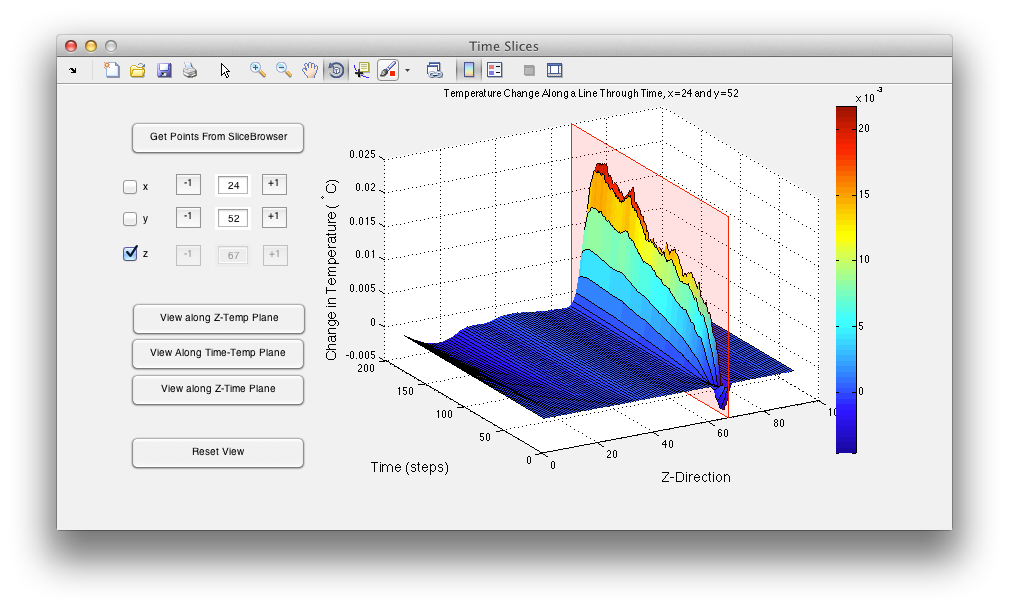
\includegraphics{tsliceplot/default-view}
    \caption[Visualization using tsliceplot]{Experimental data for activity in the motor cortex visualized with tsliceplot. \label{fig:tsliceplot}}
  \centering
\end{figure}

\begin{figure}[hbt]
  \centering
    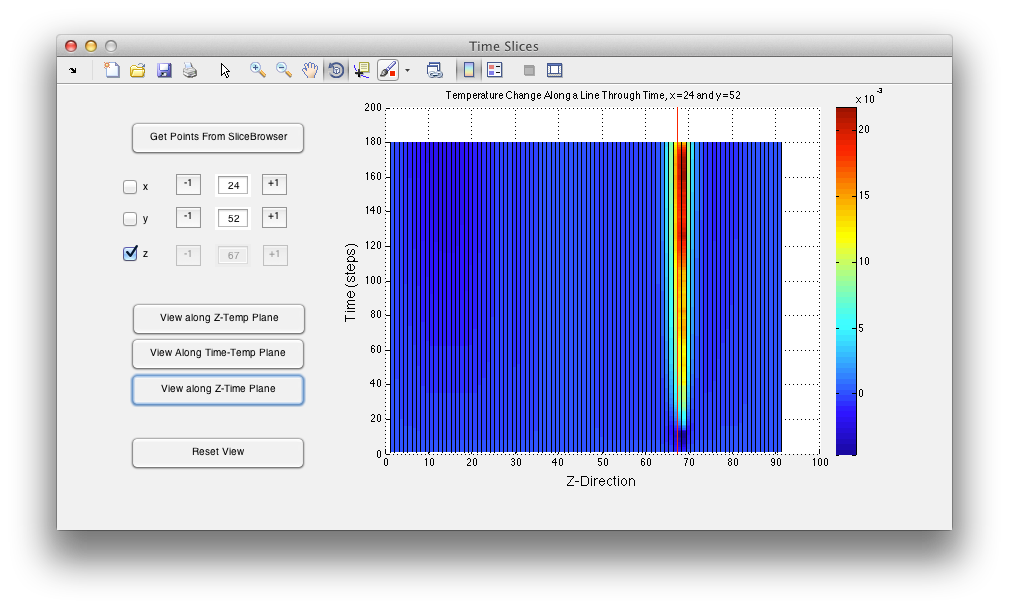
\includegraphics{tsliceplot/z-plane-view}
    \caption[Visualization using tsliceplot (z v. t plane)]{The same data as is presented in~\cref{fig:tsliceplot}, but viewed flat-on along the z vs. time plane.\label{fig:tsliceplotz}}
  \centering
\end{figure}